\documentclass[12pt]{article}

\usepackage[english]{babel}
\usepackage[letterpaper,top=2cm,bottom=2cm,left=3cm,right=3cm,marginparwidth=1.75cm]{geometry}

\title{NeoVim LaTeX Template}
\author{Benjamin Bowles}
\date{\today}

%%%%%%%%%%%%%%%%%%%
% PACKAGE IMPORTS %
%%%%%%%%%%%%%%%%%%%

\usepackage{amsmath}
\usepackage{graphicx}
\usepackage[colorlinks=true, allcolors=blue]{hyperref}


\begin{document}

%%%%%%%%%%%%%%%%%%%%%%%%%%%%%%%
\maketitle
\newpage

\tableofcontents
\newpage
%%%%%%%%%%%%%%%%%%%%%%%%%%%%%%%

%%%%%%%%%%%%%%%%%%%%%%%%%%%%%%%
\section{Figures}
% =================
\begin{figure}[ht]

\centering
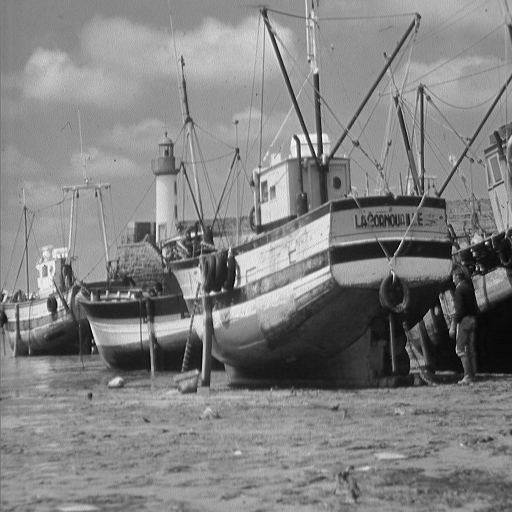
\includegraphics[width=0.5\textwidth]{figs/boat.png}
\caption{A boat}

\end{figure}
% =================
\newpage
%%%%%%%%%%%%%%%%%%%%%%%%%%%%%%%

%%%%%%%%%%%%%%%%%%%%%%%%%%%%%%%
\section{Lists}
% =================
\begin{enumerate}
    \item  Item 1
    \item  Item 2
    \item  Item 3
\end{enumerate}
\begin{itemize}
    \item  Item 1
    \item  Item 2
    \item  Item 3
\end{itemize}
% =================
\newpage
%%%%%%%%%%%%%%%%%%%%%%%%%%%%%%%

%%%%%%%%%%%%%%%%%%%%%%%%%%%%%%%
\section{Math}
% =================
\begin{equation}
    \int_{-\infty}^{\infty} e^{-x^2} dx = \sqrt{\pi}
\end{equation}
% =================
\newpage
%%%%%%%%%%%%%%%%%%%%%%%%%%%%%%%

%%%%%%%%%%%%%%%%%%%%%%%%%%%%%%%
\section{Tables}
% =================
\begin{table}[ht]
\centering
\begin{tabular}{l|r}
    Item & Price \\\hline
    widgets & 1.00 \\
    gadgets & 2.00 \\
\end{tabular}
\caption{\label{tab:widgets}A table of items and their prices}
\end{table}
% =================
\newpage
%%%%%%%%%%%%%%%%%%%%%%%%%%%%%%%

%%%%%%%%%%%%%%%%%%%%%%%%%%%%%%%
\section{Bibliographies}
% =================
\cite{TestBook}
\cite{TestArticle}

% \subsection{Bibliography}
% -----------------
\bibliography{bib}
\bibliographystyle{apalike}

% =================
\newpage
%%%%%%%%%%%%%%%%%%%%%%%%%%%%%%%

\end{document}
